\documentclass[UTF8]{ctexart}
\usepackage[a4paper,left=3cm,right=3cm,top=2cm]{geometry}
\usepackage{amsmath}
\usepackage{enumitem}
\usepackage{float}
\usepackage{threeparttable}
\usepackage{caption}
\usepackage{multirow}
\usepackage{graphicx}
\usepackage{listings}
\usepackage{xcolor}
\usepackage{amssymb}
\renewcommand{\figurename}{Figure}
\definecolor{dkgreen}{rgb}{0,0.6,0}
\definecolor{gray}{rgb}{0.5,0.5,0.5}
\definecolor{mauve}{rgb}{0.58,0,0.82}
\lstdefinelanguage{LC3}{
  morekeywords={ADD, AND, BR, BRn, BRnz, BRnzp, BRnp, BRz, BRzp, BRp, JMP, JSR, LD, LDI, LDR, LEA, NOT, ST, STI, STR},
  sensitive=false,
  morecomment=[l]{;},
  morestring=[b]",
  morekeywords=[2]{R0, R1, R2, R3, R4, R5, R6, R7}, % Define register keywords
}
\lstset{frame=tb,
  language=LC3,
  aboveskip=3mm,
  belowskip=3mm,
  showstringspaces=false,
  columns=flexible,
  basicstyle={\small\ttfamily},
  numbers=left,%设置行号位置none不显示行号
  numberstyle=\tiny\courier, %设置行号大小
  numberstyle=\tiny\color{gray},
  keywordstyle=\color{blue},
  keywordstyle=[2]\color{purple},
  commentstyle=\color{dkgreen},
  stringstyle=\color{mauve},
  breaklines=true,
  breakatwhitespace=true,
  escapeinside=`,%逃逸字符(1左面的键),用于显示中文例如在代码中`中文...`
  tabsize=4,
  extendedchars=false %解决代码跨页时,章节标题,页眉等汉字不显示的问题
}

\setlength\lineskiplimit{5.25bp}
\setlength\lineskip{5.25bp}

\title{Lab3 Report}
\author{崔士强 PB22151743}
\date{December 1, 2023}

\bibliographystyle{plain}

\begin{document}

\maketitle
\section{Purpose}
The purpose of the program is to implement strcmp() function in Language C

Anticipated outcomes:

\section{Principles}
\subsection{Overview}
The program compares two strings by conparing the ASCII value of each character. 
The starting address of string(i.e. x3100 or x3200) is read into R0 or R1. 
Then use LDR to read the data in the address and store the ASCII values respectively in R3 and R4.
If the values are the same, increment R0 and R1, then repeat the process until NULL or different ASCII values appear.
\subsection{How to compare}

After getting the ASCII values of two characters, check if both values are 0(i.e. NULL).
If yes, return zero.

Then perform substraction.
If the result is not zero, return the result, otherwise increment the registers R0 and R1.

Relevant code:
\begin{lstlisting}
LOOP        LDR         R3, R0, #0      ;Load a character in S1 into R3
            LDR         R4, R1, #0      ;Load a character in S2 into R4
            ADD         R5, R3, R4      ;If both are NULL, return #0
            BRz         RETURN_NULL
            AND         R5, R5, #0      ;Clear R5
            NOT         R4, R4
            ADD         R4, R4, #1
            ADD         R2, R3, R4      ;R3-R4
            BRnp        RETURN
            ADD         R0, R0, #1
            ADD         R1, R1, #1      ;Check the next character
            BRnzp       LOOP
\end{lstlisting}

\section{Procedure}
\subsection{Bugs encountered}
\begin{enumerate}
  \item When reading data from R0 and R1, I wrongly used LD, whose second operand cannot be a register.
  
  Solution: Use LDR instead.
\end{enumerate}

\section{Results}
Results are shown below:
\begin{figure}[h]
        \centering
        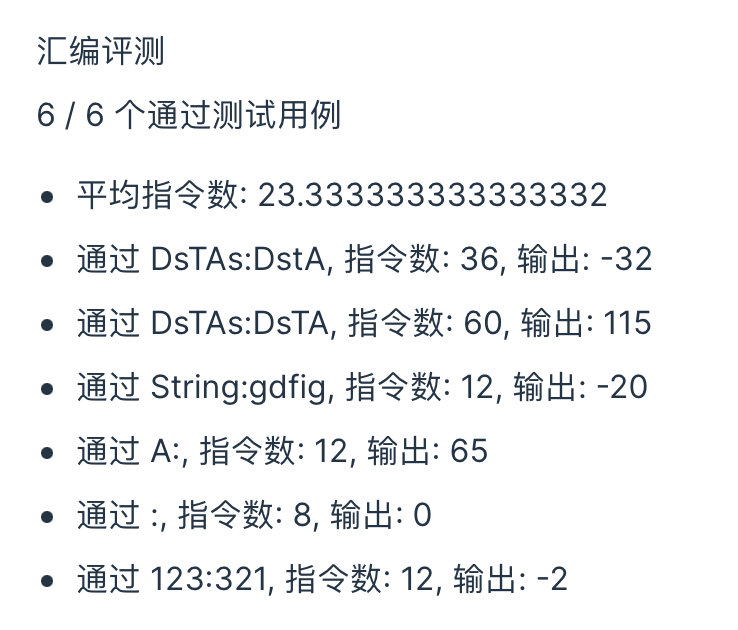
\includegraphics[scale=0.5]{result.png}
        \caption{Result}
\end{figure}

The program correctly compares various kinds of strings.

\bibliography{math}

\end{document}
\iffalse
\begin{figure}[H]
    \centering
    \includegraphics[scale=0.5]{name.png}
    \caption{name}
\end{figure}
\fi
